%\documentclass[11pt, a4paper]{article}
\documentclass[includeheaders]{scrartcl}
\usepackage{scrlayer-scrpage}
\usepackage{hyperref}
\usepackage[utf8]{inputenc}
% Deutsche Silbentrennung
\usepackage[ngermanb]{babel}
% Unterstützung für Farben
\usepackage[dvipsnames]{xcolor}
% Erweiterte Mathematik-Symbole
\usepackage{amsmath,amscd,amssymb}
% Nummerierte Listen
\usepackage{enumerate}
% Erweiterte Bildeinbettungsoptionen
\usepackage{graphicx}
% Typografisch hochwertige Tabellen
\usepackage{tabularx,ragged2e,booktabs}
% Unterstützung für Unter-Abbildungen (z.B. 2x2-Matrix)
\usepackage{float}
\usepackage{caption}
\usepackage{subcaption}
% Seitenränder
 \usepackage{geometry}
       \geometry{a4paper, 
             left=2.5cm, 
             right=2.5cm, 
             top=2.5cm, 
             bottom=2.5cm}
           
% Unterstützung für °-Zeichen
\usepackage{textcomp}
\usepackage{gensymb}
% Formatierung von \paragraph und \subparagraph anpassen
\makeatletter
\renewcommand\paragraph{\@startsection{paragraph}{4}{\z@}%
	{-3.25ex\@plus -1ex \@minus -.2ex}%
	{1.5ex \@plus .2ex}%
	{\raggedsection\normalfont\sectfont\size@paragraph}%
}
\renewcommand\subparagraph{\@startsection{subparagraph}{5}{\z@}%
	{-3.25ex\@plus -1ex \@minus -.2ex}%
	{1.5ex \@plus .2ex}%
	{\raggedsection\normalfont\sectfont\size@subparagraph\mdseries}%
}
\makeatother


\begin{document}
	
	% o - outer, i - inner, c - center -> location of header/footer-element
%\ohead{\includegraphics[scale=0.5]{img/HPI-Logo.png}}
%\ifoot{\includegraphics[scale=0.5]{img/HPI-Logo.png} }
\ifoot{\includegraphics[scale=0.07]{img/logo}}
\cfoot{Template zur Veranstaltung Modellierung II, \\ Holger Giese, Sommersemester 2016}
\ofoot{\thepage}


	
	\newpage 
	
	\title{Analysedokument\\ \small{(Veranstaltung Modellierung II, SoSe 2016)}}
	\date{}
	\author{}
	
	\maketitle
	\begin{table}[H]
		\centering
		\begin{tabular}{@{}lp{7.5cm}@{}}
			\textbf{Projekt:} & Roboterbasiertes Personentransportsystem\\
			&\\
			\textbf{Auftraggeber: }& Prof. Holger Giese \newline Hasso-Platter-Institut \newline Prof.-Dr.-Helmert-Str. 2–3 \newline 14482 Potsdam\\
			&\\
			\textbf{Auftragnehmer: }& Modellierung II – Projektgruppe 5 \\
		\end{tabular}
	\end{table}

	
	
	\newpage
	
	\begin{table}[H]
		\centering
		\begin{tabularx}{\textwidth}{@{}p{4cm}Xp{4cm}@{}}
			\toprule
			Verantwortlichkeit & Name, Vorname & Datum \\ 
			\midrule
			Ansprechpartner    & Bischoff, Sebastian & 09.05.2016 \\
			Bearbeitender      & Sauder, Jonathan & 09.05.2016 \\
			Bearbeitender      & Lüpke, Fabian & 09.05.2016 \\
			Bearbeitender      & Hering, Jonas & 09.05.2016 \\
			Bearbeitender      & Braun, Jakob & 09.05.2016  \\
			Bearbeitender      & Cremerius, Jonas & 09.05.2016 \\
			Bearbeitender      & Wischner, Jakob & 09.05.2016 \\
			Bearbeitender      & Schwenkert, Daniel & 09.05.2016 \\
			Bearbeitender      & Jäkel, Dominik & 09.05.2016 \\
			Bearbeitender      & König, Bastian & 09.05.2016 \\
			\bottomrule
		\end{tabularx}
	\end{table}
	
	\vspace{2cm}
	
	\tableofcontents
	
	\newpage
	
	\section{Zielbestimmung}
	Die Aufgabe des Projektteams ist es ein System zu entwickeln, das selbstfahrender Roboter in einer Stadt der Zukunft koordiniert. In dieser Stadt existieren keine Straßen mehr – umso komplexer wird der Prozess das Navigationsverhalten der Roboter mit den richtigen Parametern einzustellen und zu modellieren. Die Voraussetzungen und Spezifikation dafür zu erfassen ist Ziel dieser Analyse – die sich insbesondere mit dem Fahr- und dem Aufladevorgang der Roboter und ihren Manövrierfähigkeiten gegenüber Hindernissen auseinandersetzt.

	Im weiteren Verlauf des Projektes sollen die Roboter ebenfalls Krankentransporter und schließlich Bestandteil eines Taxiservicedienstes werden. Alle hier getroffenen Annahmen, Modellierungen und Implementierungen könnten damit im Rahmen der späteren Anwendungen revidiert werden.

	Als Ausgangspunkt stellt das Unternehmen eine unbegrenzte Anzahl von Robotern zur Verfügung, die mit Aktoren, Sensoren und einem Ortungsgerat ausgestattet sind, und im Wechselspiel mit einem Server agieren.

	Das Primärziel des Projektes ist es dabei ein möglichst effizientes Transportsystem zu entwickeln, um für alle Verkehrsbegebenheiten im Großraum einer Zukunftsstadt vorbereitet zu sein. Davon würde die Zielgruppe Mensch nachhaltig profitieren, indem Verkehrsunfällen, Staus und die zeitliche Inanspruchnahme des Fahrens auf ein Minimum reduziert werden. Allerdings wird das System zuerst vor einige Probleme im Fahrvorgang gestellt, mit denen sich die folgenden Kapitel beschäftigen – werden sie gelöst, könnte langfristig ein einzelnes Unternehmen die gesamte Transportinfrastruktur einer Großstadt Übernehmen. Das System wird von sich aus selbstständig und vollständig autonom agieren. Abgesehen davon Sicherheitsregeln einzuhalten, sollten damit keine Vorkenntnisse für die Fahrt mit den Robotern notwendig sein, um den Personennahvekehr für die breite Masse zu öffnen. 
	
	\pagebreak
	
	\section{Produkteinsatz}
	
		\subsection{Beschreibung des Problembereichs}
		Der Problembereich lässt sich für diese Analysestufe in drei Punkte einteilen, um eine Gesamtkoordination effizient zu gestalten:

		\begin{enumerate}
		\item
			Zuallererst muss das automatische Fahren im zweidimensionalen
			Koordinatensystem zu einem angegebenen Zielpunkt(\emph{Destination})
			fehlerfrei möglich sein. Ebenfalls steht eine manuelle Steuerung zur
			Verfügung, um unerwarteten Ereignissen zu begegnen, die allerdings
			wiederum sinnvoll in das Gesamtsystem integriert werden muss.
		\item
			Als zweite Herausforderung geht es darum den Schaden von Kollisionen
			zu minimieren; wie diese erkannt, wie auf sie reagiert wird und diese
			Kollisionen durch vorrauschendes Umfahren von
			Objekten (\emph{Obstacle}) verhindert werden können. Dies schließt
			sowohl bewegliche Objekte als auch unbewegliche Objekte mit ein.
		\item
			Im dritten Punkt gilt es einen möglichst reibungs- und
			unterbrechungslosen Batteriebetrieb zu garantieren, um zeitlich
			vorrauschendes Fahren zu ermöglichen. Im Falle eines niedrigen
			Batteriestands also unverzüglich an seiner individuellen Ladestation 
			(\emph{Charger}) anzudocken und aufzuladen, beziehungsweise längere
			Fahrten nicht anzutreten, die den Batteriestand gefährden würden.
		\end{enumerate}

		\begin{figure}[H]
			\centering
			\begin{subfigure}[t]{0.3\textwidth}
				\includegraphics[width=\textwidth]{../images/grafikZumProblembereich1.jpg}
				\caption{Fahren zu einem angegebenen Zielpunkt}
				\label{fig:2-1-problembereich-1}
			\end{subfigure}
			~~~~
			\begin{subfigure}[t]{0.3\textwidth}
				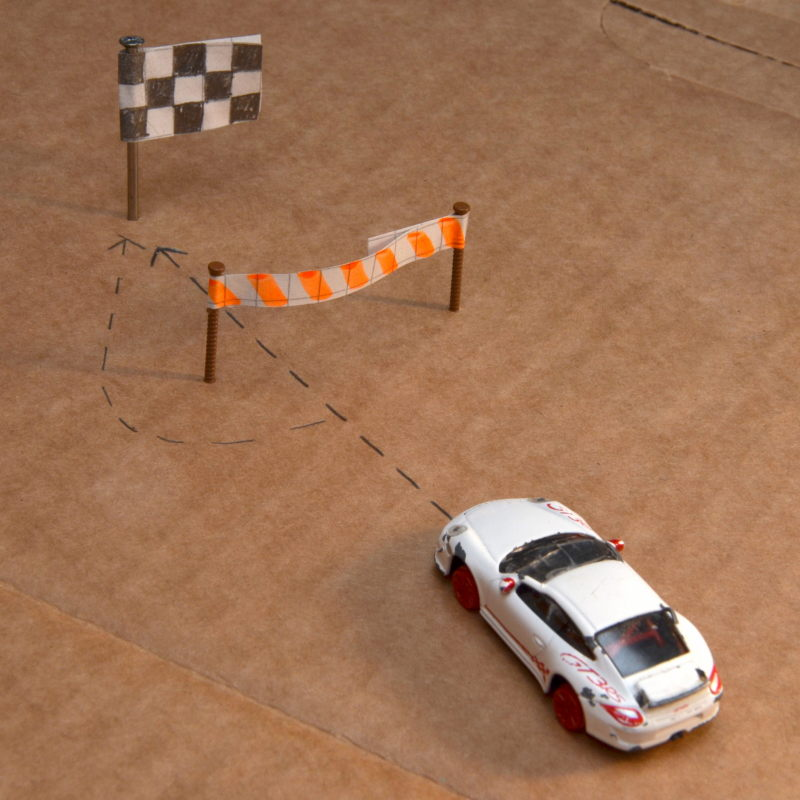
\includegraphics[width=\textwidth]{../images/grafikZumProblembereich2.jpg}
				\caption{Umfahren von Objekten}
				\label{fig:2-1-problembereich-2}
			\end{subfigure}
			~~~~
			\begin{subfigure}[t]{0.3\textwidth}
				\includegraphics[width=\textwidth]{../images/grafikZumProblembereich3.jpg}
				\caption{Automatisches Laden}
				\label{fig:2-1-problembereich-3}
			\end{subfigure}
			\caption{Visualisierung der Problembereiche}\label{fig:2-1-problembereiche}
		\end{figure}

		Abbildung \ref{fig:2-1-problembereiche} zeigt die drei o.g. Problembereiche in einer fotografischen Repräsentation.\\
	

		Daran anknüpfend wird mit folgenden Annahmen gearbeitet:

		\begin{enumerate}
		\item
			Zur Vereinfachung des Fahrverhalten muss jedes Zielobjekt physisch
			erreichbar sein. Ziele sind dementsprechend keine Hindernisse, das
			gleiche gilt für Ladestationen.
		\item
			Roboter können autark vom \emph{Server} agieren, damit ihre Ziele
			bestimmen und eine Ladestation anfahren.
		\item
			Bei den beweglichen Objekten wird davon ausgegangen, dass es sich im
			Verkehrsbetrieb ausschließlich um andere Roboter handelt. Für die
			unbeweglichen Objekte ist es notwendig, dass ihre Position von
			vornerein bekannt ist und sie unverändert bleibt.
		\end{enumerate}
		
		\subsection{Glossar}

		% \begin{description}
		% 	\item[Robot]{Roboter, der sich im 2-Dimensionalen Raum bewegen kann.}
		% 	\item[Server]{Verteilt Aufträge an die Roboter}
		% 	\item[Charger]{Ladestation für den Roboter}
		% 	\item[Destination]{Vom Server verwaltete Ziele, die der Roboter ansteuern kann.}
		% 	\item[Obstacle]{Hindernisse, die der Roboter erkennt und umfährt.}
		% \end{description}

		\begin{table}[H]
			\centering
			\begin{tabularx}{\textwidth}{@{}p{3cm}X@{}}
				\toprule
				Begriff & Erklärung\\ 
				\midrule
				Robot & Roboter, der sich im 2-Dimensionalen Raum bewegen
				kann.\\
				Server & Verteilt Aufträge an die Roboter\\
				Charger & Ladestation für den Roboter\\
				Destination & Vom Server verwaltete Ziele, die der Roboter ansteuern
				kann.\\
				Obstacle & Hindernisse, die der Roboter erkennt und
				umfährt\\
				\bottomrule
			\end{tabularx}
			\label{tab:2-2-glossar}
		\end{table}
		
		\subsection{Modell des Problembereichs}
		Abbildung \ref{fig:2-3-modell-problembereich} zeigt ein Klassendiagramm, welches das Modell des Problembereichs grafisch darstellt.
		\begin{figure}[H]
			\centering
			\includegraphics[width=0.8\textwidth]{../images/Problembereich.pdf}
			\caption{Klassendiagramm des Problembereichs}
			\label{fig:2-3-modell-problembereich}
		\end{figure}
		
		\subsection{Beschreibung der Geschäftsprozesse}
		
			\subsubsection*{Beschreibung zu 1: Choose Robot}

			\begin{table}[H]
				\centering
				\begin{tabularx}{\textwidth}{@{}p{3cm}X@{}}
				\toprule
				\textbf{Auslösendes Ereignis:} & Der Server will den für ein bestimmtes Ziel bestmöglichen Roboter auswählen und diesen zum Ziel schicken. \\ \midrule
				\textbf{Ergebnis:} & Alle Roboter haben ihre Sensordaten ausgelesen und diese dem Server
				mitgeteilt. Daraufhin hat der Server einen Roboter ausgewählt, der für
				die Zielanfahrung optimal geeignet ist, und diesem den Auftrag zum
				Anfahren des Ziels übermittelt. \\ \midrule
				\textbf{Mitwirkende:} &	Server, Roboter \\
				\bottomrule
				\end{tabularx}
				\label{tab:2-4-choose-robot}
			\end{table}

			Abbildung \ref{fig:2-4-choose-robot-aktivitaetendiagramm} zeigt ein Aktivitätendiagramm, welches den Ablauf des Geschäftsprozesses \emph{1: Choose Robot} darstellt.
			\begin{figure}[H]
				\centering
				\includegraphics[width=\textwidth]{../images/Iteration0_Analyse_2-4_chooseRobot.pdf}
				\caption{Illustration von \emph{1: Choose Robot} durch Aktivitätendiagramm}
				\label{fig:2-4-choose-robot-aktivitaetendiagramm}
			\end{figure}

			Um den für ein gegebenes Ziel bestmöglichen \emph{Robot} auszuwählen, sendet
			der \emph{Server} zunächst an alle \emph{Robots} eine Anfrage (\emph{request}),
			woraufhin die \emph{Robots} ihre Sensordaten (\emph{sensor data}) auslesen und
			an den \emph{Server} senden. Auf Grundlage dieser Daten wählt der \emph{Server} den
			\emph{Robot} aus, der für die Zielanfahrung optimal positioniert ist und
			sendet ihm die konkrete Aufforderung (\emph{task}) zum Anfahren des
			Ziels.

			Wie die Sensordaten und der Algorithmus zur Wahl des optimalen \emph{Robots}
			konkret definiert sind, ist eine Entwurfsentscheidung, die zum Zeitpunkt
			dieser ersten Ausbaustufe noch nicht getroffen wurde.

			\subsubsection*{Beschreibung zu 2: Drive to Destination}

			\begin{table}[H]
				\centering
				\begin{tabularx}{\textwidth}{@{}p{3cm}X@{}}
				\toprule
				\textbf{Auslösendes Ereignis:} & Ein \emph{Robot} hat eine \emph{Destination} erhalten.\\ \midrule
				\textbf{Ergebnis:} & Der \emph{Robot} ist unter Umfahrung von womöglichen \emph{Obstacles} zur \emph{Destination} gefahren.\\ \midrule
				\textbf{Mitwirkende:} &	Ein einzelner, autonomer \emph{Robot}. \\
				\bottomrule
				\end{tabularx}
				\label{tab:2-4-drive-to-destination}
			\end{table}

			Abbildung \ref{fig:2-4-drive-to-destination-aktivitaetendiagramm} zeigt ein Aktivitätendiagramm, welches den Ablauf des Geschäftsprozesses \emph{2: Drive to Destination} darstellt.
			
			\begin{figure}[H]
				\centering
				%\includegraphics[width=\textwidth]{../images/Iteration0_Analyse_2-4_chooseRobot.pdf}
				\caption{Illustration von \emph{1: choose Robot} durch Aktivitätendiagramm}
				\label{fig:2-4-drive-to-destination-aktivitaetendiagramm}
			\end{figure}

			Dieser Prozess wird autonom vom \emph{Robot} ausgeführt. Er wird genau
			dann ausgeführt, wenn der Roboter eine \emph{Destination} vom Server
			erhalten hat, die er anfahren soll. Da der \emph{Robot} an dieser Stelle
			dem Server schon bestätigt hat, dass sein Akkustand hoch genug ist, ist
			der einzige Sonderfall, den wir betrachten müssen, dass ein
			\emph{Obstacle} auf der direkten Linie zwischen \emph{Robot} und
			\emph{Destination} liegt. Dann wird der \emph{Robot} nach Wahl des
			besten Umweges das \emph{Obstacle} umfahren und wieder die Fahrt zur
			\emph{Destination} Aufnehmen.
			
	\pagebreak
	
	\section{Produktfunktionen}
	% \input{3-Produktfunktionen}
	
		\subsection{Use Cases}
		% \input{3-1-Use_Cases}
		
		\subsection{Beschreibung zu Use Case \emph{1}: Drive to Destination}

			\subsubsection*{Charakterisierende Informationen}

			\begin{table}[H]
				\centering
				\begin{tabularx}{\textwidth}{@{}p{5cm}X@{}}
				\toprule
				\textbf{Übergeordneter elementarer Geschäftsprozess:} & Drive to Destination\\ \midrule
				\textbf{Ziel des Use Cases:} & \emph{Robot} fährt ein Ziel an\\ \midrule
				\textbf{Umgebende Systemgrenze:} & \emph{Robot} \\ \midrule
				\textbf{Vorbedingung:} & Ein spezieller \emph{Robot} wurde vom Server ausgewählt und sein Akkustand ist hoch genug um den Auftrag auszuführen \\ \midrule
				\textbf{Nachbedingung bei erfolgreicher Ausführung:} & \emph{Robot} ist am Ziel angekommen und meldet dies dem \emph{Server} \\ \midrule
				\textbf{Beteiligte Nutzer:} & \emph{Robot} \\ \midrule
				\textbf{Auslösendes Ereignis:} & \emph{Robot} hat eine \emph{Destination} erhalten. \\ 
				\bottomrule
				\end{tabularx}
			\end{table}

			Dieser Use Case wird dann benutzt, wenn ein \emph{Robot} ein aktuelles
			Ziel hat. In dieser Ausbaustufe betrachten wir lediglich das Anfahren
			eines Ziels von einem Roboter. Der Roboter dreht sich zunächst in die
			Richtung des Ziels und fährt so lange in Luftlinie, bis er entweder
			ankommt oder ein Hindernis erkennt. Ein konkreter Prozess zur Erkennung
			eines Hindernisses ist eine Entwurfsentscheidung und wird daher noch
			nicht berücksichtigt. Wenn der \emph{Robot} ein Hindernis erkennt, dann
			sucht er einen guten Weg um das Hindernis herum. Wie er diesen Weg sucht
			ist auch zunächst eine Entwurfsentscheidung und noch nicht relevant. Auf
			diesem Weg umfährt er dann das Hindernis und nimmt erneut die Fahrt auf
			Luftlinie auf.
			
			\subsubsection*{Szenario für den Standardablauf (Erfolg)}

			\begin{table}[H]
				\centering
				\begin{tabularx}{\textwidth}{@{}cp{2cm}X@{}}
				\toprule
				Schritt & Nutzer & Beschreibung der Aktivität \\ \midrule
				1 & Robot & \emph{Robot} dreht sich in Richtung aktueller \emph{Destination} \\
				2 & Robot & \emph{Robot} fährt geradeaus \\
				3 & Robot & \emph{Robot} erreicht \emph{Destination} \\
				\bottomrule
				\end{tabularx}
			\end{table}
			
			\subsubsection*{Szenarien für alternative Abläufe\\ (Misserfolg oder Umwege zum Erfolg)}

			\begin{table}[H]
				\centering
				\begin{tabularx}{\textwidth}{@{}cp{6cm}X@{}}
				\toprule
				Schritt & Bedingung für Alternative & Beschreibung der Aktivität \\ \midrule
				3 & \emph{Robot} erkennt ein Hindernis zwischen auf seinem Weg zum Ziel & \emph{Robot} sucht sich einen Umweg um das Hindernis, umfährt das Hindernis und nimmt schließlich Standardablauf wieder auf \\
				\bottomrule
				\end{tabularx}
			\end{table}

			%\subsubsection*{Beschreibung des allgemeinen Ablaufes}

		\subsection{Beschreibung zu Use Case \emph{2}: Read Sensors}

			\subsubsection*{Charakterisierende Informationen}

			\begin{table}[H]
				\centering
				\begin{tabularx}{\textwidth}{@{}p{5cm}X@{}}
				\toprule
				\textbf{Übergeordneter elementarer Geschäftsprozess:} & Choose Robot\\ \midrule
				\textbf{Ziel des Use Cases:} & \emph{Robot} kann über seinen Akkustand und seine Position Auskunft geben\\ \midrule
				\textbf{Umgebende Systemgrenze:} & \emph{Robot} \\ \midrule
				\textbf{Vorbedingung:} & \emph{Robot} hat eine Anfrage vom Server erhalten \\ \midrule
				\textbf{Nachbedingung bei erfolgreicher Ausführung:} & \emph{Robot} schickt die ermittelten Informationen an den Server \\ \midrule
				\textbf{Beteiligte Nutzer:} & \emph{Robot} \\ \midrule
				\textbf{Auslösendes Ereignis:} & \emph{Robot} hat eine Anfrage vom Server erhalten, seine Sensoren zu lesen und sie dem Server zu schicken \\ 
				\bottomrule
				\end{tabularx}
			\end{table}

			Im Rahmen vom Geschäftsprozess \emph{Choose Robot} sammelt der Server
			Informationen über jeden \emph{Robot}. Diese Informationen (z.B
			Akkustand, aktuelle Position, ob der Roboter gerade ein Ziel verfolgt)
			kann der Roboter von seinen Hardware-Schnittstellen anfordern. Dieses
			Use Case wird dann ausgefüht, wenn der \emph{Robot} eine Anfrage vom
			Server erhält, seine Sensoren zu lesen, und endet damit, dass der Robot
			die zusammengefassten Informationen an den Server schickt.
			
			\subsubsection*{Szenario für den Standardablauf (Erfolg)}

			\begin{table}[H]
				\centering
				\begin{tabularx}{\textwidth}{@{}cp{2cm}X@{}}
				\toprule
				Schritt & Nutzer & Beschreibung der Aktivität \\ \midrule
				1 & Robot & \emph{Robot} erhält Anfrage vom Server \\
				2 & Robot & \emph{Robot} sammelt Informationen von seiner Hardwareschnittstelle und fasst sie zusammen \\
				3 & Robot & \emph{Robot} schickt zusammengefasste Informationen an den Server \\
				\bottomrule
				\end{tabularx}
			\end{table}

			%\subsubsection*{Beschreibung des allgemeinen Ablaufes}

		\subsection{Beschreibung zu Use Case \emph{3}: Read Sensors}

			\subsubsection*{Charakterisierende Informationen}

			\begin{table}[H]
				\centering
				\begin{tabularx}{\textwidth}{@{}p{5cm}X@{}}
				\toprule
				\textbf{Übergeordneter elementarer Geschäftsprozess:} & Drive to destination\\ \midrule
				\textbf{Ziel des Use Cases:} & Ziel ist es, dem Robot zu ermöglichen seine Ladestation anzufahren\\ \midrule
				\textbf{Umgebende Systemgrenze:} & Robot\\ \midrule
				\textbf{Nachbedingung bei erfolgreicher Ausführung:} & Der Robot muss sein vorgegebenes Ziel erreichen\\ \midrule
				\textbf{Beteiligte Nutzer:} & Robot\\ \midrule
				\textbf{Auslösendes Ereignis:} & Robot erreicht Ziel (Use-Case)\\ 
				\bottomrule
				\end{tabularx}
			\end{table}

			Jedem Robot wird, laut Aufgabenstellung, eine feste Ladestation zugewiesen. Der Robot fährt vollständig autonom diese Ladestation an. Daher ist keine Kommunikation mit dem Server notwendig.
			
			\subsubsection*{Szenario für den Standardablauf (Erfolg)}

			\begin{table}[H]
				\centering
				\begin{tabularx}{\textwidth}{@{}cp{2cm}X@{}}
				\toprule
				Schritt & Nutzer & Beschreibung der Aktivität \\ \midrule
				1 & Robot & \emph{Robot} erreicht Ziel \\
				2 & Robot & \emph{Robot} fährt zur Ladestation \\
				3 & Robot & \emph{Robot} erreicht Ladestation und lädt sich auf \\
				4 & Robot & \emph{Robot} erhält neues Ziel und fährt dorthin \\
				\bottomrule
				\end{tabularx}
			\end{table}

			%\subsubsection*{Beschreibung des allgemeinen Ablaufes}

		\subsection{Beschreibung zu Use Case \emph{4}: Choose Robot}

			\subsubsection*{Charakterisierende Informationen}

			\begin{table}[H]
				\centering
				\begin{tabularx}{\textwidth}{@{}p{5cm}X@{}}
				\toprule
				\textbf{Übergeordneter elementarer Geschäftsprozess:} & \\ \midrule
				\textbf{Ziel des Use Cases:} & passenden \emph{Robot} für die durch den \emph{Server} gesendete \emph{Destination} auswählen\\ \midrule
				\textbf{Umgebende Systemgrenze:} & \emph{Robot} und \emph{Server} \\ \midrule
				\textbf{Vorbedingung:} & \emph{Server} hat eine neue \emph{Destination} bekommen\\ \midrule
				\textbf{Nachbedingung bei erfolgreicher Ausführung:} & dem ausgewählten \emph{Robot} wird die Task übertragen\\ \midrule
				\textbf{Beteiligte Nutzer:} & \emph{Robot} und \emph{Server}\\ \midrule
				\textbf{Auslösendes Ereignis:} & \emph{Server} empfängt neue \emph{Destination}\\ 
				\bottomrule
				\end{tabularx}
			\end{table}
			
			\subsubsection*{Szenario für den Standardablauf (Erfolg)}

			\begin{table}[H]
				\centering
				\begin{tabularx}{\textwidth}{@{}cp{2cm}X@{}}
				\toprule
				Schritt & Nutzer & Beschreibung der Aktivität \\ \midrule
				1 & Server & \emph{Server} sendet Anfragen an alle \emph{Robots} \\
				2 & Robot & \emph{Robots} empfangen Anfrage und führen dann den Use-Case „read Sensor“ aus \\
				3 & Robot & \emph{Robots} senden ihre ermittelten Sensorwerte an den \emph{Server}\\
				4 & Server & \emph{Server} empfängt Daten und wählt den am Besten geeigneten \emph{Robot} aus \\
				\bottomrule
				\end{tabularx}
			\end{table}

			%\subsubsection*{Beschreibung des allgemeinen Ablaufes}

		\subsection{Beschreibung zu Use Case \emph{5}: Assign Task}

			\subsubsection*{Charakterisierende Informationen}
 
			\begin{table}[H]
				\centering
				\begin{tabularx}{\textwidth}{@{}p{5cm}X@{}}
				\toprule
				\textbf{Übergeordneter elementarer Geschäftsprozess:} & \\ \midrule
				\textbf{Ziel des Use Cases:} & \emph{Robot} den Task (die \emph{Destination}) zuweisen\\ \midrule
				\textbf{Umgebende Systemgrenze:} & \emph{Server} und \emph{Robot} \\ \midrule
				\textbf{Vorbedingung:} & „choose Robot“ hat am Besten geeigneten \emph{Robot} gefunden und ausgewählt\\ \midrule
				\textbf{Nachbedingung bei erfolgreicher Ausführung:} & ausgewähler \emph{Robot} steuert die \emph{Destination} an\\ \midrule
				\textbf{Beteiligte Nutzer:} & \emph{Server} und \emph{Robot}\\ \midrule
				\textbf{Auslösendes Ereignis:} & im Use-Case „choose Robot“ wurde passender \emph{Robot} ausgewählt\\ 
				\bottomrule
				\end{tabularx}
			\end{table}
			
			\subsubsection*{Szenario für den Standardablauf (Erfolg)}

			\begin{table}[H]
				\centering
				\begin{tabularx}{\textwidth}{@{}cp{2cm}X@{}}
				\toprule
				Schritt & Nutzer & Beschreibung der Aktivität \\ \midrule
				1 & Server & \emph{Server} überträgt ausgewähltem \emph{Robot} den Task \\
				\bottomrule
				\end{tabularx}
			\end{table}

			%\subsubsection*{Beschreibung des allgemeinen Ablaufes}
			
	\pagebreak
			
	\section{Produktumgebung}
	% \input{4-Produktumgebung}
	
		\subsection{Systemumgebung}
		Im nachfolgenden Abschnitt werden die bekannten Komponenten des Systems
		und die dazugehörigen Schnittstellen beschrieben. Grundsätzlich besteht
		das System aus mindestens einem \emph{Robot}, hierfür geeigneten
		\emph{Chargern} und einem zentralen \emph{Server}.
		
			\subsubsection{Hardwareumgebung}
			\paragraph{Server}\label{server}

			Es existiert ein zentraler \emph{Server}. Dieser \emph{Server} verfügt
			über ausreichende Ressourcen und ist in der Lage direkt mit den
			Transportvehikeln zu kommunizieren.

			\subparagraph{IServerCore}\label{iservercore}

			Der \emph{Server} verfügt über einen zentralen Hauptprozessor, über den
			auf alle weiteren Komponenten zugegriffen werden kann. Dies wird der
			Einfachheit halber angenommen.

			\subparagraph{IServerMessageHandler}\label{iservermessagehandler}

			Mit der Kommunikationseinheit \emph{IServerMessageHandler} kann der
			\emph{Server} Nachrichten direkt an einen \emph{Robot} senden. Der
			Einfachheit wegen wird angenommen, die Komponente ist stets
			empfangsbereit und die dahinterstehende Infrastruktur zur Übertragung
			von Nachrichten stabil.

			\paragraph{Robot}\label{robot}

			Das Transportvehikel \emph{Robot} erfüllt Grundfunktionalitäten wie das
			Anfahren von Zielen, das Umfahren von Hindernissen und das Laden des
			Akkumulators. Nachfolgend werden die zentralen Hardwarekomponenten des
			\emph{Robots} beschrieben.

			\subparagraph{IRobotCore}\label{irobotcore}

			Der \emph{Robot} verfügt über einen zentralen Hauptprozessor, über den
			auf alle weiteren Komponenten zugegriffen werden kann. Dies wird der
			Einfachheit halber angenommen.

			\subparagraph{IRobotMessageHandler}\label{irobotmessagehandler}

			Mit der Kommunikationseinheit \emph{IRobotMessageHandler} kann der
			\emph{Robot} Nachrichten, die vom zentralen \emph{Server} für das
			Vehikel abgesetzt wurden, direkt empfangen.

			\subparagraph{IRobotEngine}\label{irobotengine}

			Als Antrieb nutzt das Transportvehikel einen omnidirektionalen Antrieb
			mit 3 Motoren, über welchen es sich vorwärts, nach rechts, nach links
			oder durch Drehen um die eigene Achse bewegen lässt. Der Antrieb
			ermöglich eine Fahrt in verschiedenen Geschwindigkeiten, wobei eine
			nicht näher spezifizierte Grenze nicht überschritten werden kann.

			\subparagraph{IBattery}\label{ibattery}

			Jeder \emph{Robot} verfügt über einen Akkumulator, der zur
			Energieversorgung dient. Eine ausreichende Ladung des Akkumulators ist
			deshalb zum Betrieb des \emph{Robot} unbedingt erforderlich. Der
			Akkumulator hat eine maximale Ladekapazität und kann über einen
			\emph{Charger} geladen werden. Die genaue Beschaffenheit des
			Akkumulators ist nicht bekannt.

			\subparagraph{INorthStar}\label{inorthstar}

			Die Komponente \emph{INorthStar} kann ähnlich einem GPS-Modul die
			Position des \emph{Robots} feststellen. Hierbei ist die Komponente in
			der Lage, die Koordinaten der Position in einem zweidimensionalen
			Koodinatensystem und die aktuelle Ausrichtung des Vehikels zu ermitteln.

			\subparagraph{IRSensorDistance}\label{irsensordistance}

			Das Transportvehikel verfügt über 9 Infarotdistanzsensoren, die an der
			kreisförmigen Außenwand des Vehikels im Abstand von jeweils 40
			angeordnet sind. Über sie ist die Feststellung der Entfernung des
			Vehikels von allen bewegten und unbewegten Objekten in der Umgebung
			möglich.

			\subparagraph{IBumper}\label{ibumper}

			Bei einer Kollision des \emph{Robots} mit einem anderen Objekt wird
			dieses Ereignis über die Sensorik eine Kollisionserkennung, worauf
			weitere Schritte eingeleitet werden können.

			\paragraph{Charger}\label{charger}

			Es existieren Ladestationen, über die sich die \emph{IBattery} der
			\emph{Robots} vollständig laden lässt. Eine Ladestation ist dabei genau
			einem \emph{Robot} zugeordnet. Zum Laden muss ein \emph{Robot} seine
			Ladestation anfahren, worauf die Ladung sofort beginnt. Jede Ladestation
			verfügt über eine genaue Position.
			
			\subsubsection{Softwareumgebung}
			\paragraph{Server}\label{server}

			Auf dem \emph{Server} läuft, da nicht anders angegeben, ein
			Standard-Betriebssystem. Darauf läuft eine Laufzeitumgebung, die die
			benötigten Methoden zur Kommunikation mit den Robots bereitstellt. Die
			wichtigste (und einzige bisher spezifizierte) Methode, ist die
			CallRobot() Methode um einen \emph{Robot} anzurufen und einen
			Datenaustausch herzustellen.

			\subparagraph{IServerMessageHandler}\label{iservermessagehandler}

			Der \emph{IServerMessageHandler} ist die Komponente, die ausgehende
			Informationen des \emph{Servers} für einen \emph{Robot} versendet. Das
			Verhalten und die enthaltenen Methoden sind dabei allerdings nicht näher
			spezifiziert.

			\paragraph{Robot}\label{robot}

			Nachfolgend werden die zentralen Softwareschnittstellen des
			\emph{Robots} beschrieben.

			\subparagraph{IRobotCore}\label{irobotcore}

			Auf der zentralen Recheneinheit des \emph{Robots}, dem
			\emph{IRobotCore}, läuft eine JavaRuntimeEnvironment, in der sich die
			gesamte Steuerung und die Verwendung der Komponenten und Schnittstellen
			abspielt. Die einzelnen Komponenten mit ihren Methoden werden im
			folgenden näher erläutert.

			\subparagraph{IRSensorDistance}\label{irsensordistance}

			Die \emph{IRSensorDistance} Komponente stellt drei Methoden bereit, mit
			denen die Distanz und der Winkel des entdeckten Objekts und der an der
			Entdeckung beteiligte Infrarotsensor erfasst und in Arrays gespeichert
			werden.

			\subparagraph{IDistanceSensor}\label{idistancesensor}

			Die besagten Arrays kann der \emph{IDistanceSensor} auslesen. Er hat
			dazu ebenfalls drei Methoden. getIRDistances() gibt ein Array mit allen
			erfassten Objekten zurück, getIRDistancesInRange() gibt ebenfalls ein
			Array zurück, das allerdings nur die Objekte in einem gewissen Abstand
			enthält und getNearestIRDistances() gibt nur das nächste Objekt zurück.

			\subparagraph{INorthStar}\label{inorthstar}

			Die Komponente \emph{INorthStar} ist für die Positionierung zuständig
			und greift dabei auf ein Device zur Standortbestimmung zurück. Sie hat
			zwei Methoden. Eine liest die aktuelle Position aus, die andere die
			aktuelle Ausrichtung. Die Position besteht dabei aus zwei float-Werten,
			einer x- und einer y-Koordinate.

			\subparagraph{IRobotMessageHandler}\label{irobotmessagehandler}

			Der \emph{IRobotMessageHandler} ist die Komponente, die eintreffende
			Anrufe des \emph{Servers} verarbeitet. Das Verhalten und die enthaltenen
			Methoden sind dabei allerdings nicht näher spezifiziert. So kann man
			davon ausgehen, dass jegliche Methoden der anderen Komponenten über den
			\emph{IRobotCore} aufgerufen und die Ergebnisse an die
			\emph{IMessageHandler} Komponente übergeben werden können, damit diese
			die Informationen auf Anfrage des \emph{Servers} beschaffen und
			übermitteln kann.

			\subparagraph{IBumperHandler}\label{ibumperhandler}

			Die \emph{IBumperHandler} ist die Komponente zum Umgang mit
			Zusammenstößen. Die Kollisionserkennung \emph{IBumper} registriert einen
			Aufprall und die \emph{IBumperHandler} Komponente stellt zwei Methoden
			zum Umgang mit dem Aufprall bereit.

			\subparagraph{IDrive}\label{idrive}

			Die Bewegungssteuerung des Robots heißt \emph{IDrive}. Sie stellt vier
			Methoden bereit. Die Methoden driveToPosition() und
			driveToPositionCautiously() erwarten beide eine Position, eine
			Geschwindigkeit und einen ArrivalHandler, der eine Methode zur Meldung
			aufruft, wenn der \emph{Robot} am Ziel angekommen ist. Die Methoden sind
			beide dafür da, ein gegebenes Ziel anzufahren, wobei bei der Zweiten die
			Höchstgeschwindigkeit geringer ist. Die höchstgeschwindigkeit für
			Cautiously, Regular und Fast Methoden stellt die \emph{IDrive}
			Komponente bereit, wobei Cautiously $\leq$ Regular $\leq$ Fast gilt.\\
			Die anderen beiden Methoden, drive() und driveCautiously() unterscheiden
			sich ebenfalls nur in der Höchstgeschwindigkeit und ermöglichen ein
			manuelles Fahren. Dabei erwarten sie die Drehung des \emph{Robots} als
			float-Wert sowie die Vorwärts- und die Seitwärtsgeschwindigkeit,
			ebenfalls als float-Wert.

			\subparagraph{IBattery}\label{ibattery}

			Bei \emph{IBattery} handelt es sich um die Akkusteuerung des
			\emph{Robots}. Sie stellt zwei Methoden bereit. getBatteryLevel() gibt
			den aktuellen Akkuladestand als float-Wert zurück, getChargingPosition()
			gibt die Position des zugeordneten \emph{Chargers} zurück.

			\subsubsection{Ressourcenübersicht}
			In Abbildung \ref{fig:4-1-3-verteilungsdiagramm} werden die in 4.1.1 und 4.1.2 beschriebenen
			Komponenten und Schnittstellen im Verteilungsdiagramm dargestellt.

			\begin{figure}[H]
				\centering
				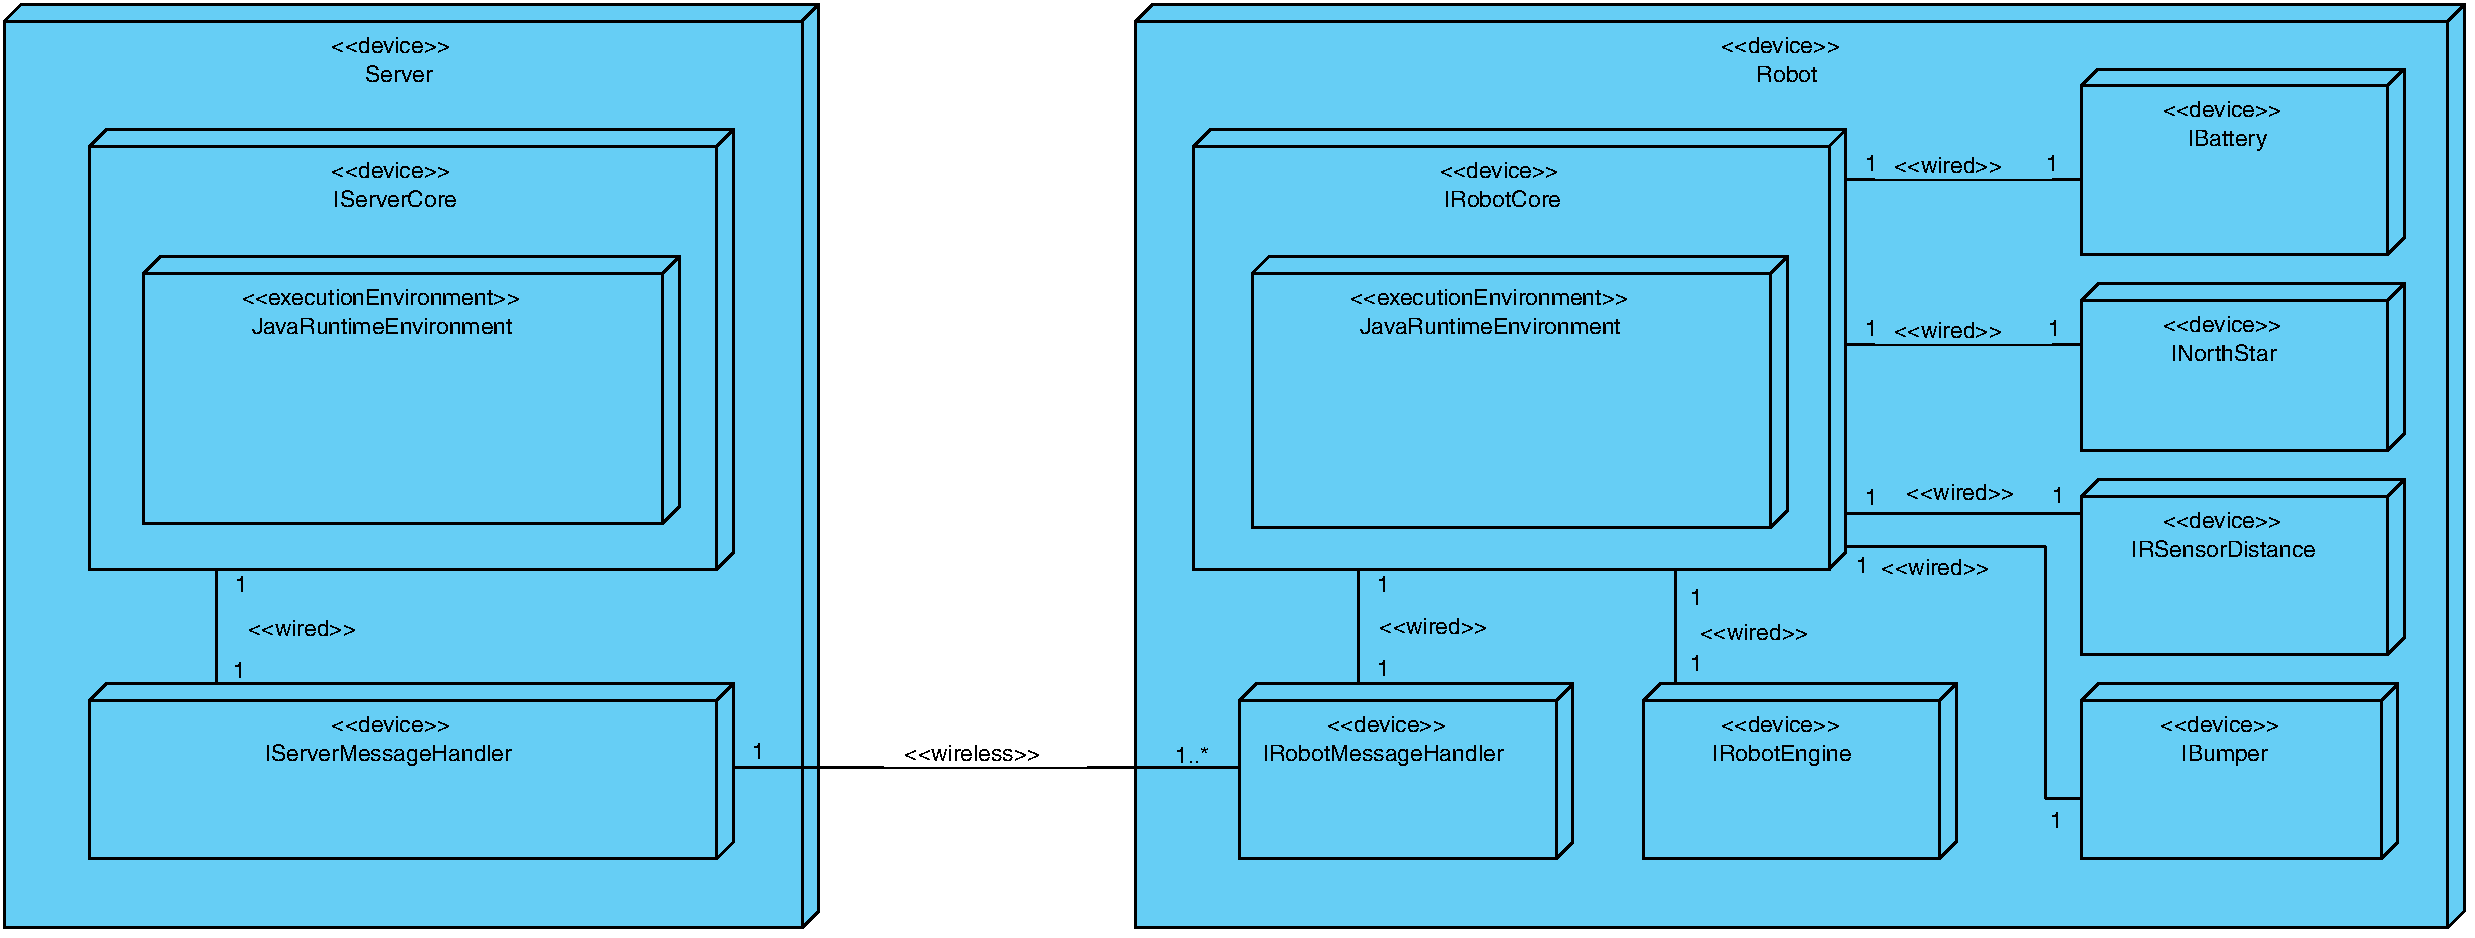
\includegraphics[width=1.5\textwidth, angle=90]{../images/Iteration0_Analyse_4-1-3_ressourcenuebersicht.pdf}
				\caption{Verteilungsdiagramm}
				\label{fig:4-1-3-verteilungsdiagramm}
			\end{figure}
					
\end{document}